\chapter{Prototipo desarrollado} \chapterlabel{Primer_prototipo} \label{cap:prototipo1v2}

\section{Introducción}\label{sec:introProto1}

Como se mencionó previamente, el proyecto se llevó a cabo en forma incremental. Esta modalidad consiste en desarrollar núcleos pequeños que, una vez completados, evolucionan mediante el agregado de nuevas funcionalidades y el mejoramiento de aquellas que ya poseían.

Se realizaron dos prototipos. El primero de ellos se enfocó en lograr la lectura de la patente, la detección de la presencia del vehículo y la manipulación de una barrera, considerando una sola vía de acceso.

Una vez que este primer módulo se puso a punto, se mejoraron algunas de sus funcionalidades y se le añadieron nuevas, dando lugar al segundo prototipo. 


\section{Prototipo inicial}

En la etapa inicial del proyecto se desarrolló un primer prototipo cuyo objetivo principal fue lograr la correcta obtención las patentes de los vehículos detectados. Por este motivo, en esta fase no se tuvieron en cuenta varios aspectos que se presentan en un escenario real, como por ejemplo, la diferenciación entre vía de ingreso y de egreso.

Durante la realización de este prototipo se desarrollaron tres códigos en lenguaje C++, uno para la UCC, otro para el módulo WiFi y un tercero para la Placa I/O. El primero de ellos fue diseñado en el entorno de desarrollo Eclipse \cite{eclipse}, el cual es una plataforma de software compuesto por un conjunto de herramientas de programación de código abierto y multiplataforma. Por otra parte, los otros dos códigos fueron desarrollados mediante el IDE (Integrated Development Environment) de Arduino \cite{arduinoide}, debido a que tanto el microcontrolador como el módulo WiFi utilizados son compatibles con el software que provee esta compañía.

A continuación, se detalla el funcionamiento de este primer prototipo.
En primer lugar, se lleva a cabo una etapa de conexión entre el módulo WiFi, la Placa I/O y la UCC. En esta, al encender el sistema, la Placa I/O pone en alto el pin de reset del módulo WiFi produciendo el arranque del mismo.

Una vez encendido, el módulo procede a conectarse a la red WiFi local creada mediante un router y, luego, genera un servidor web en su dirección IP. A partir de este momento, la placa y el módulo quedan a la espera de que la UCC se conecte a dicho servidor. La primera acción que esta última lleva a cabo es la creación un socket TCP/IP, el cual utiliza para conectarse al servidor mencionado anteriormente. De esta manera, se concluye la etapa de conexión y el sistema queda listo para funcionar en modo continuo.

Cuando se presiona alguno de los dos pulsadores, acción que representa la detección de un vehículo mediante uno de los sensores magnéticos, el microcontrolador de la Placa I/O recibe dicha información y se la envía por puerto serie al módulo WiFi. Este último, comunica la información sobre el estado de los magnéticos a la UCC vía WiFi, únicamente si alguno de ellos fue activado. 

Entonces, cuando a la UCC le llega esta información, a partir del procesamiento de los trabajos generados por el OpenALPR, se obtiene la patente del vehículo detectado.

En esta etapa, la activación de cualquiera de los pulsadores por separado, o de ambos simultáneamente, desemboca en la misma condición: la activación del sistema de reconocimiento de patentes sin discriminación entre entrada o salida. Esto se debe a que aún no se desarrolló esta distinción, ya que el principal objetivo de este primer prototipo es la verificación del correcto funcionamiento del reconocimiento. Luego de que se obtuvo la patente, la Unidad Central se la envía a la Placa I/O, de manera de indicarle que levante la barrera.

Cabe destacar que los tres códigos fueron desarrollados de manera secuencial. Esto implica que, si por ejemplo se activa algún detector magnético mientras se lleva a cabo un proceso de ingreso o egreso anterior, el sistema no podrá responder a dicho evento.



\section{Prototipo final}

En esta sección, se desarrollará el funcionamiento del prototipo final del proyecto. En este, la principal modificación fue la coexistencia de dos vías, una de ingreso y otra de egreso, funcionando simultáneamente. Para realizar esto se utilizó el software YAKINDU Statecharts Tools \cite{yakinduprincipalpage} con una licencia académica, la cual brinda acceso a todas sus funcionalidades seis meses. Además, su entorno de desarrollo está basado en Eclipse, lo que facilitó su uso, ya que dicho software fue implementado al realizar el prototipo inicial.

Este framework es capaz de generar bloques de código en diferentes lenguajes tales como C, C++ o Java, a partir de una máquina de estado conformada mediante diagramas UML (Unified Modeling Language). En la figura~\ref{fig:img_statemachintable} se presenta una tabla comparativa entre las máquinas de estado UML y otros tipos, donde se observan las ventajas que las primeras poseen sobre las demás.

\begin{figure}[H]
	\centering
	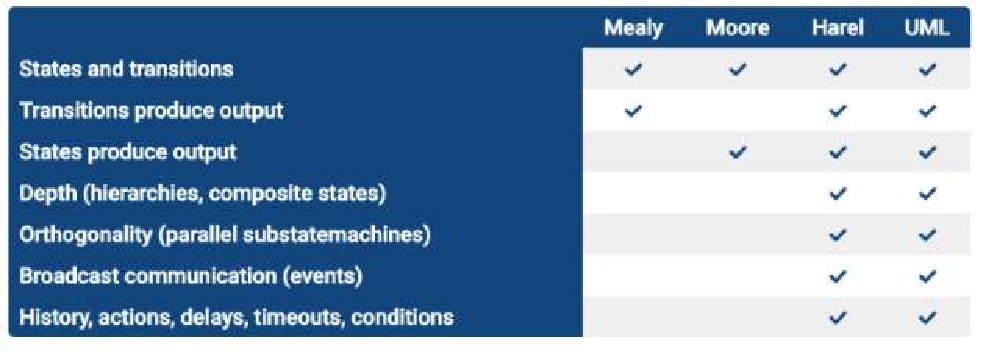
\includegraphics[width=\textwidth]{statemachintable.pdf}
	\caption{Comparación entre diferentes máquinas de estado \cite{yakindustatemachine}.}
	\label{fig:img_statemachintable}
\end{figure}

Los sistemas diseñados a partir de esta herramienta tienen dos formas de funcionamiento: basadas en ciclos o basadas en eventos \cite{yakinduevent-cycle}. Para cualquiera de los dos casos, un ciclo es el procedimiento mediante el cual el sistema analiza si debe pasar o no al siguiente estado, en cada una de las regiones que posea. La diferencia entre éstas dos formas de funcionamiento radica en el disparador del siguiente ciclo. En el primer caso, el sistema ejecuta su siguiente ciclo cada un cierto periodo de tiempo fijo, mientras que en la segunda forma, se espera a que algún evento haya ocurrido para ejecutar el ciclo. Debido a que en este proyecto se requiere que determinadas acciones sucedan a lo largo del ingreso o egreso para poder avanzar, se ha diseñado un sistema basado en eventos.

Por otra parte, mediante esta herramienta es posible generar sistemas basados en la técnica de la multiprogramación, es decir, la ejecución de tareas de manera concurrente por el procesador a tal velocidad que causa la impresión de ser en paralelo. Esto es de vital importancia para poder considerar a la entrada y la salida como dos vías independientes, permitiendo efectuar ambos procesos simultáneamente. Además, al igual que el entorno de Eclipse, este software permite el desarrollo de proyectos de Arduino, que pueden ser cargados sobre las placas de dicha compañía. Debido a estas razones, tanto el código de la UCC como el de la Placa I/O fueron desarrollados mediante esta herramienta. Cabe destacar que el código correspondiente al módulo WiFi se generó con el IDE de Arduino, ya que no presentó gran complejidad debido a que únicamente es un intermediario entre la UCC y la placa. En la figura~\ref{fig:img_diagrama-comunicacion} se puede observar un diagrama en bloques representativo de la comunicación dentro del sistema.

\begin{figure}[H]
	\centering
	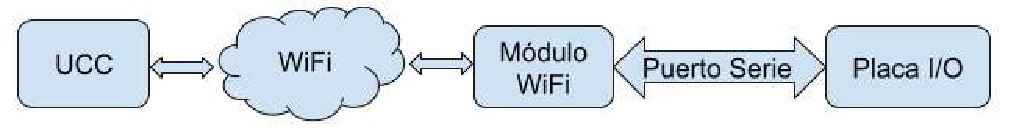
\includegraphics[width=\textwidth]{diagrama-comunicacion.pdf}
	\caption{Comunicación entre UCC, Módulo y Placa.}
	\label{fig:img_diagrama-comunicacion}
\end{figure}

En las siguientes secciones de este capítulo se desarrollará el funcionamiento de cada una de las etapas del sistema.  Se destaca que, a pesar de que su funcionamiento se explique en forma individual, las mismas trabajan en forma conjunta, a excepción de la fase de conexión.
  

\subsection{Fase de conexión}

En esta primera etapa, se busca establecer la conexión entre la UCC, el módulo WiFi y la Placa I/O. Esta fase ocurre solamente al iniciaro el sistema.

Cada uno de los códigos desarrollados con el software YAKINDU posee una región específica para esta etapa, y las mismas se pueden observar en las figuras \ref{fig:img_ConexionPlaca} y \ref{fig:img_ConexionUCC}. Por otra parte, en el módulo WiFi, esto sucede dentro del setup de Arduino, como se ve en la figura~\ref{fig:img_setupmodwifi}. 

\begin{figure}[H]
	\centering
	\begin{subfigure}[b]{0.49\textwidth}
		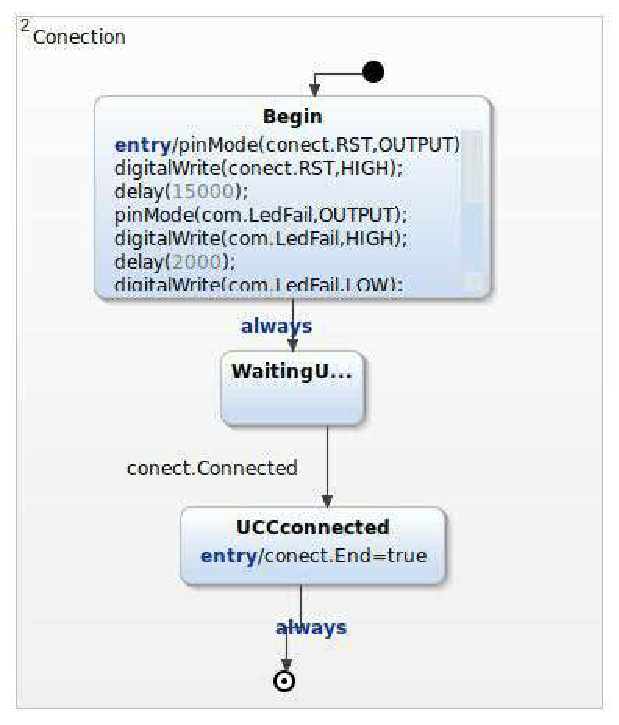
\includegraphics[width=\textwidth]{ConexionPlaca.pdf}
		\caption{Región de conexión de Placa I/O.}
		\label{fig:img_ConexionPlaca}
	\end{subfigure}
	\hfill
	\begin{subfigure}[b]{0.49\textwidth}
		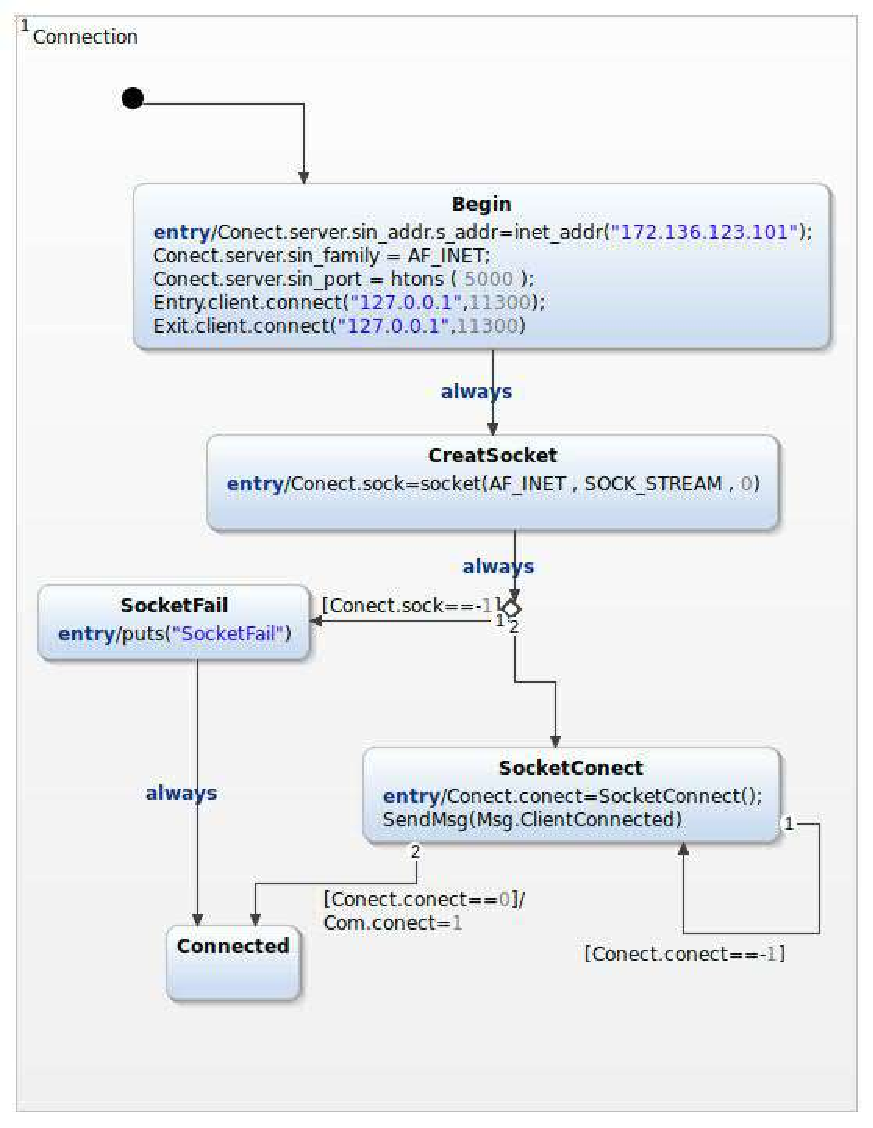
\includegraphics[width=\textwidth]{ConexionUCC.pdf}
		\caption{Región de conexión de UCC.}
		\label{fig:img_ConexionUCC}
	\end{subfigure}
	\hfill
	\begin{subfigure}[b]{0.49\textwidth}
		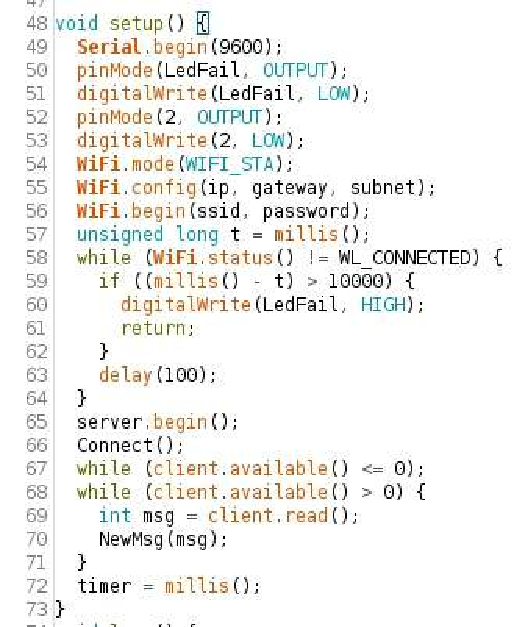
\includegraphics[scale=0.7]{setupmodwifi.pdf}
		\caption{Conexión del módulo WiFi.}
		\label{fig:img_setupmodwifi}
	\end{subfigure}
	\caption{Proceso de establecimiento de la conexión entre UCC, módulo WiFi y Placa I/O.}
\end{figure}

Al encender la Placa I/O, el microcontrolador pone en alto uno de sus pines digitales, el cual se encuentra conectado al pin de reset del módulo WiFi. De esta manera, el funcionamiento de este último queda controlado por la placa. Debido a que al iniciar el módulo el mismo escribe caracteres residuales en su puerto serie, la placa tiene un tiempo de espera de 15 segundos antes de inicializar dicha comunicación. De esta manera, se evita que estos caracteres afecten el funcionamiento normal de la placa. Luego de este período, esta última permanece a la espera de que se establezca la conexión por parte de la UCC.

Como se observa en la figura~\ref{fig:img_setupmodwifi}, luego de iniciar, el módulo WiFi se conecta a la red WiFi que se le indica, crea un servidor web y queda a la espera de que la UCC se conecte al mismo. En caso de no poder conectarse a la red correspondiente, el módulo encenderá un led que indica la existencia de una falla.

Por su parte, la UCC debe conectarse al servidor creado. Para esto, luego de inicializar las variables necesarias, procede a crear un socket TCP/IP y conectarse a través de este al servidor. Es preciso mencionar que, en caso de falla en la creación o en la conexión del socket, el sistema informa dichos errores en pantalla.

Una vez establecida la conexión, la UCC le envía un mensaje al módulo WiFi indicándole este suceso, terminando su parte en la etapa de conexión. Al recibirlo, el módulo lo reenvía a la placa, poniendo fin a la etapa de conexión en su totalidad. De esta manera, el sistema queda preparado para su funcionamiento en forma continua. Se debe tener en cuenta que si se inicializa el código de la UCC en simultáneo con la placa, este mensaje que se envía se pierde. Esto se debe a los 15 segundos de demora establecidos en el microcontrolador para iniciar la comunicación serie. Por tal motivo, luego de este tiempo, la placa enciende durante dos segundos su led de falla, indicando que está preparada para la recepción de mensajes. Entonces, el código de la UCC debe ejecutarse luego de la ocurrencia de este evento.


\subsection{Envío y recepción de mensajes}

En los tres sistemas, al recibir un mensaje, este es contestado por el receptor con un mensaje de ACK para confirmar su llegada. Debe aclararse que los mensajes de ACK recibidos no se contestan. Por otra parte, al enviar un mensaje diferente de ACK, todos los sistemas deben recibir su respectivo mensaje de confirmación. De esta manera, se puede comprobar el arribo de todos los mensajes que se envían de un punto a otro. En caso de que un mensaje de ACK no se reciba en el plazo de 10 segundos establecido, se enciende un led de falla o se muestra un mensaje de error en pantalla, dependiendo de qué sistema no lo recibió. Ante una falla de este tipo, se determinó que el sistema deje de funcionar. A futuro, se implementará una solución que no implique reiniciar el sistema manualmente.

El envío y recepción de mensajes es la función principal del módulo WiFi, ya que se encarga de tomar los mensajes provenientes de un extremo y enviarlos al otro. Por lo tanto, el módulo no es más que un intermediario entre la placa y la UCC.

Por su parte, la Unidad Central posee una región especial que se encarga de comprobar si todos los ACK fueron recibidos correctamente.  La misma se activa cada vez que en alguna parte del código se ejecuta la función de envío de mensajes. Esto puede observarse en la figura~\ref{fig:img_WaitACKUCC}.

\begin{figure}[H]
	\centering
	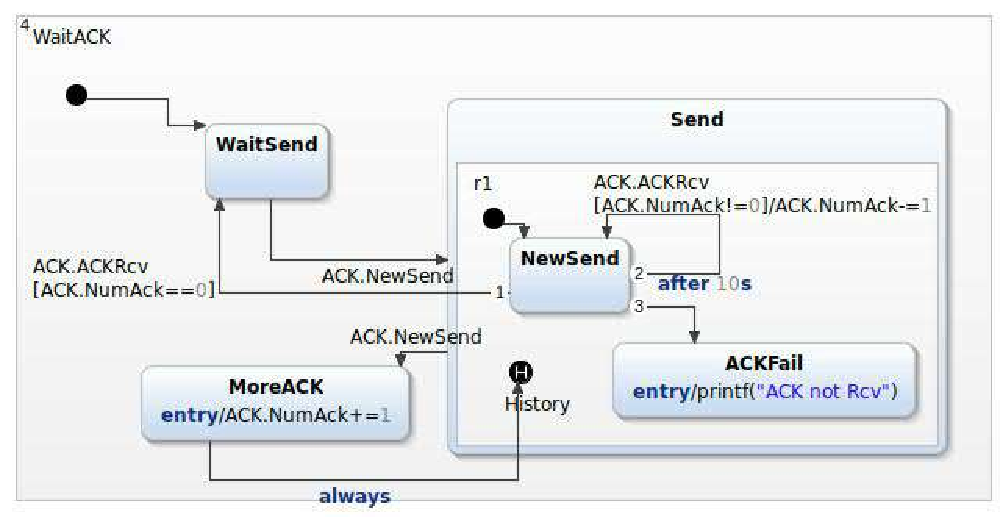
\includegraphics[width=\textwidth]{WaitACKUCC.pdf}
	\caption{Control de ACK de la UCC.}
	\label{fig:img_WaitACKUCC}
\end{figure}

En cuanto a la recepción de mensajes, la UCC se encuentra continuamente verificando si llegó alguno nuevo. En caso de que esto ocurra, informa en pantalla lo que recibió y procede a ejecutar las acciones que correspondan, ya sea modificar algún valor, levantar algún evento, entre otras.

Por otra parte, la Placa I/O posee dos regiones, una destinada a la recepción de mensajes y otra para el envío de los mismos. Estas pueden observarse en las figuras~\ref{fig:img_RcvMSGPlaca} y \ref{fig:img_SendMSGPlaca}, respectivamente.

\begin{figure}[H]
	\centering
	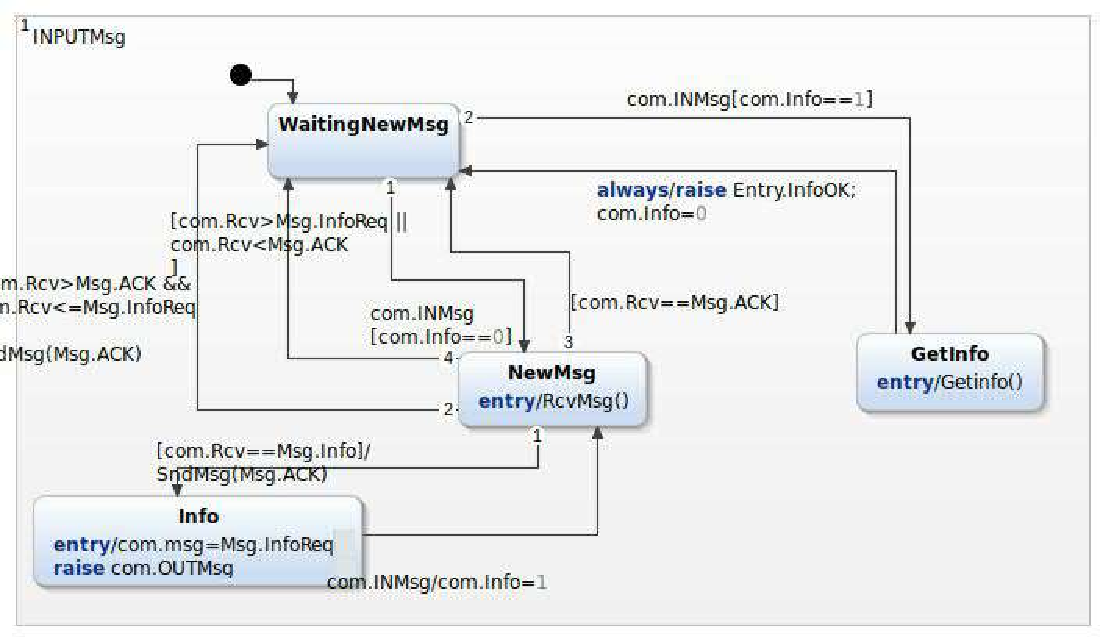
\includegraphics[width=\textwidth]{RcvMSGPlaca.pdf}
	\caption{Recepción de mensajes desde Placa I/O.}
	\label{fig:img_RcvMSGPlaca}
\end{figure}

\begin{figure}[H]
	\centering
	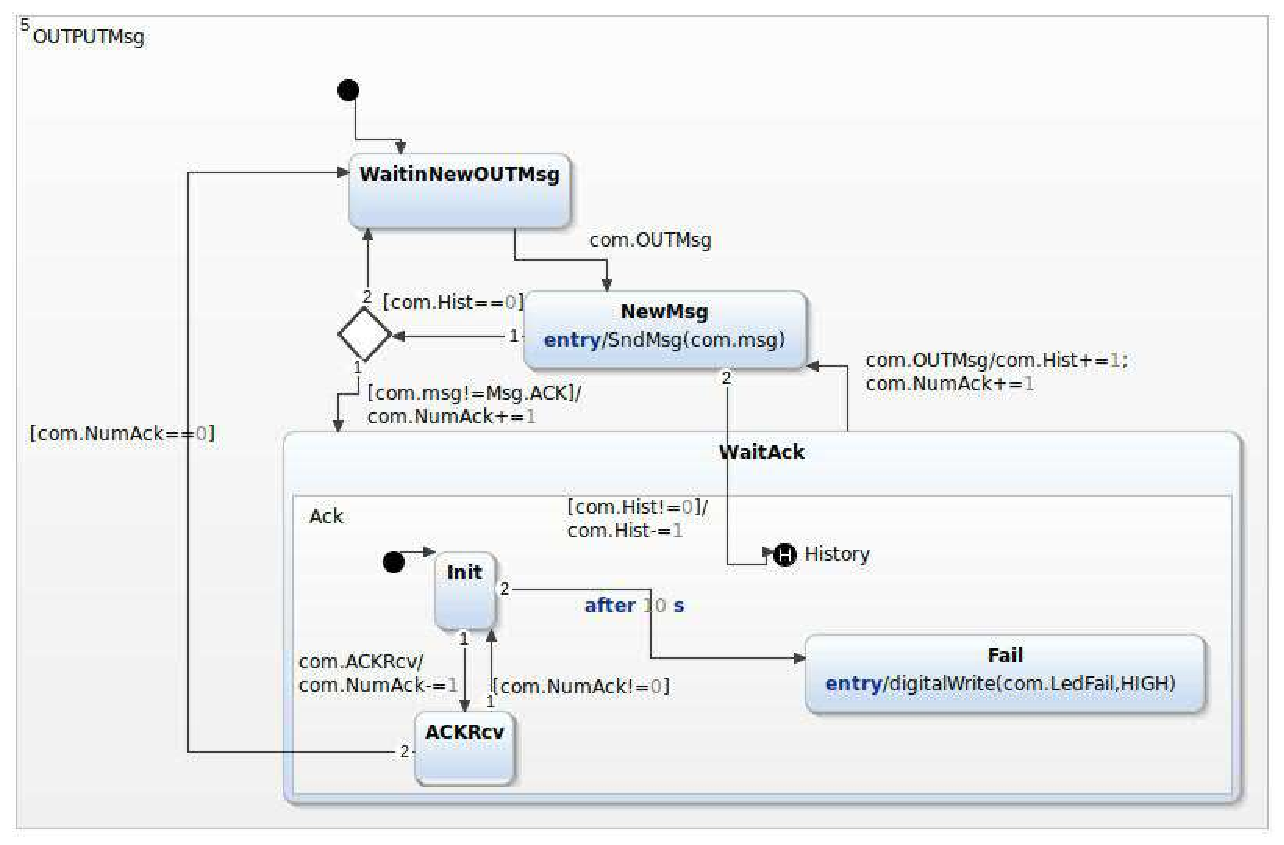
\includegraphics[width=\textwidth]{SendMSGPlaca.pdf}
	\caption{Envío de mensajes desde Placa I/O.}
	\label{fig:img_SendMSGPlaca}
\end{figure}

En la figura~\ref{fig:img_RcvMSGPlaca}, se pueden observar las diferentes reacciones del sistema ante la recepción de un ACK, de la información del vehículo o cualquiera de los otros posibles mensajes. Por otra parte, en la región de envío de mensajes, se puede visualizar el estado WaitACK, donde el sistema comprueba el arribo de ACKs para los mensajes que haya enviado.


\subsection{Vía de ingreso}

Tanto la UCC como la Placa I/O disponen de una región destinada al funcionamiento de la vía de ingreso al establecimiento.  Éstas dos se pueden observar en las figuras~\ref{fig:img_EntradaUCC} y~\ref{fig:img_EntradaPlaca}, respectivamente. Por su parte, durante esta etapa, el módulo WiFi solo envía los mensajes que recibe, de un extremo al otro.

\begin{figure}[H]
	\centering
	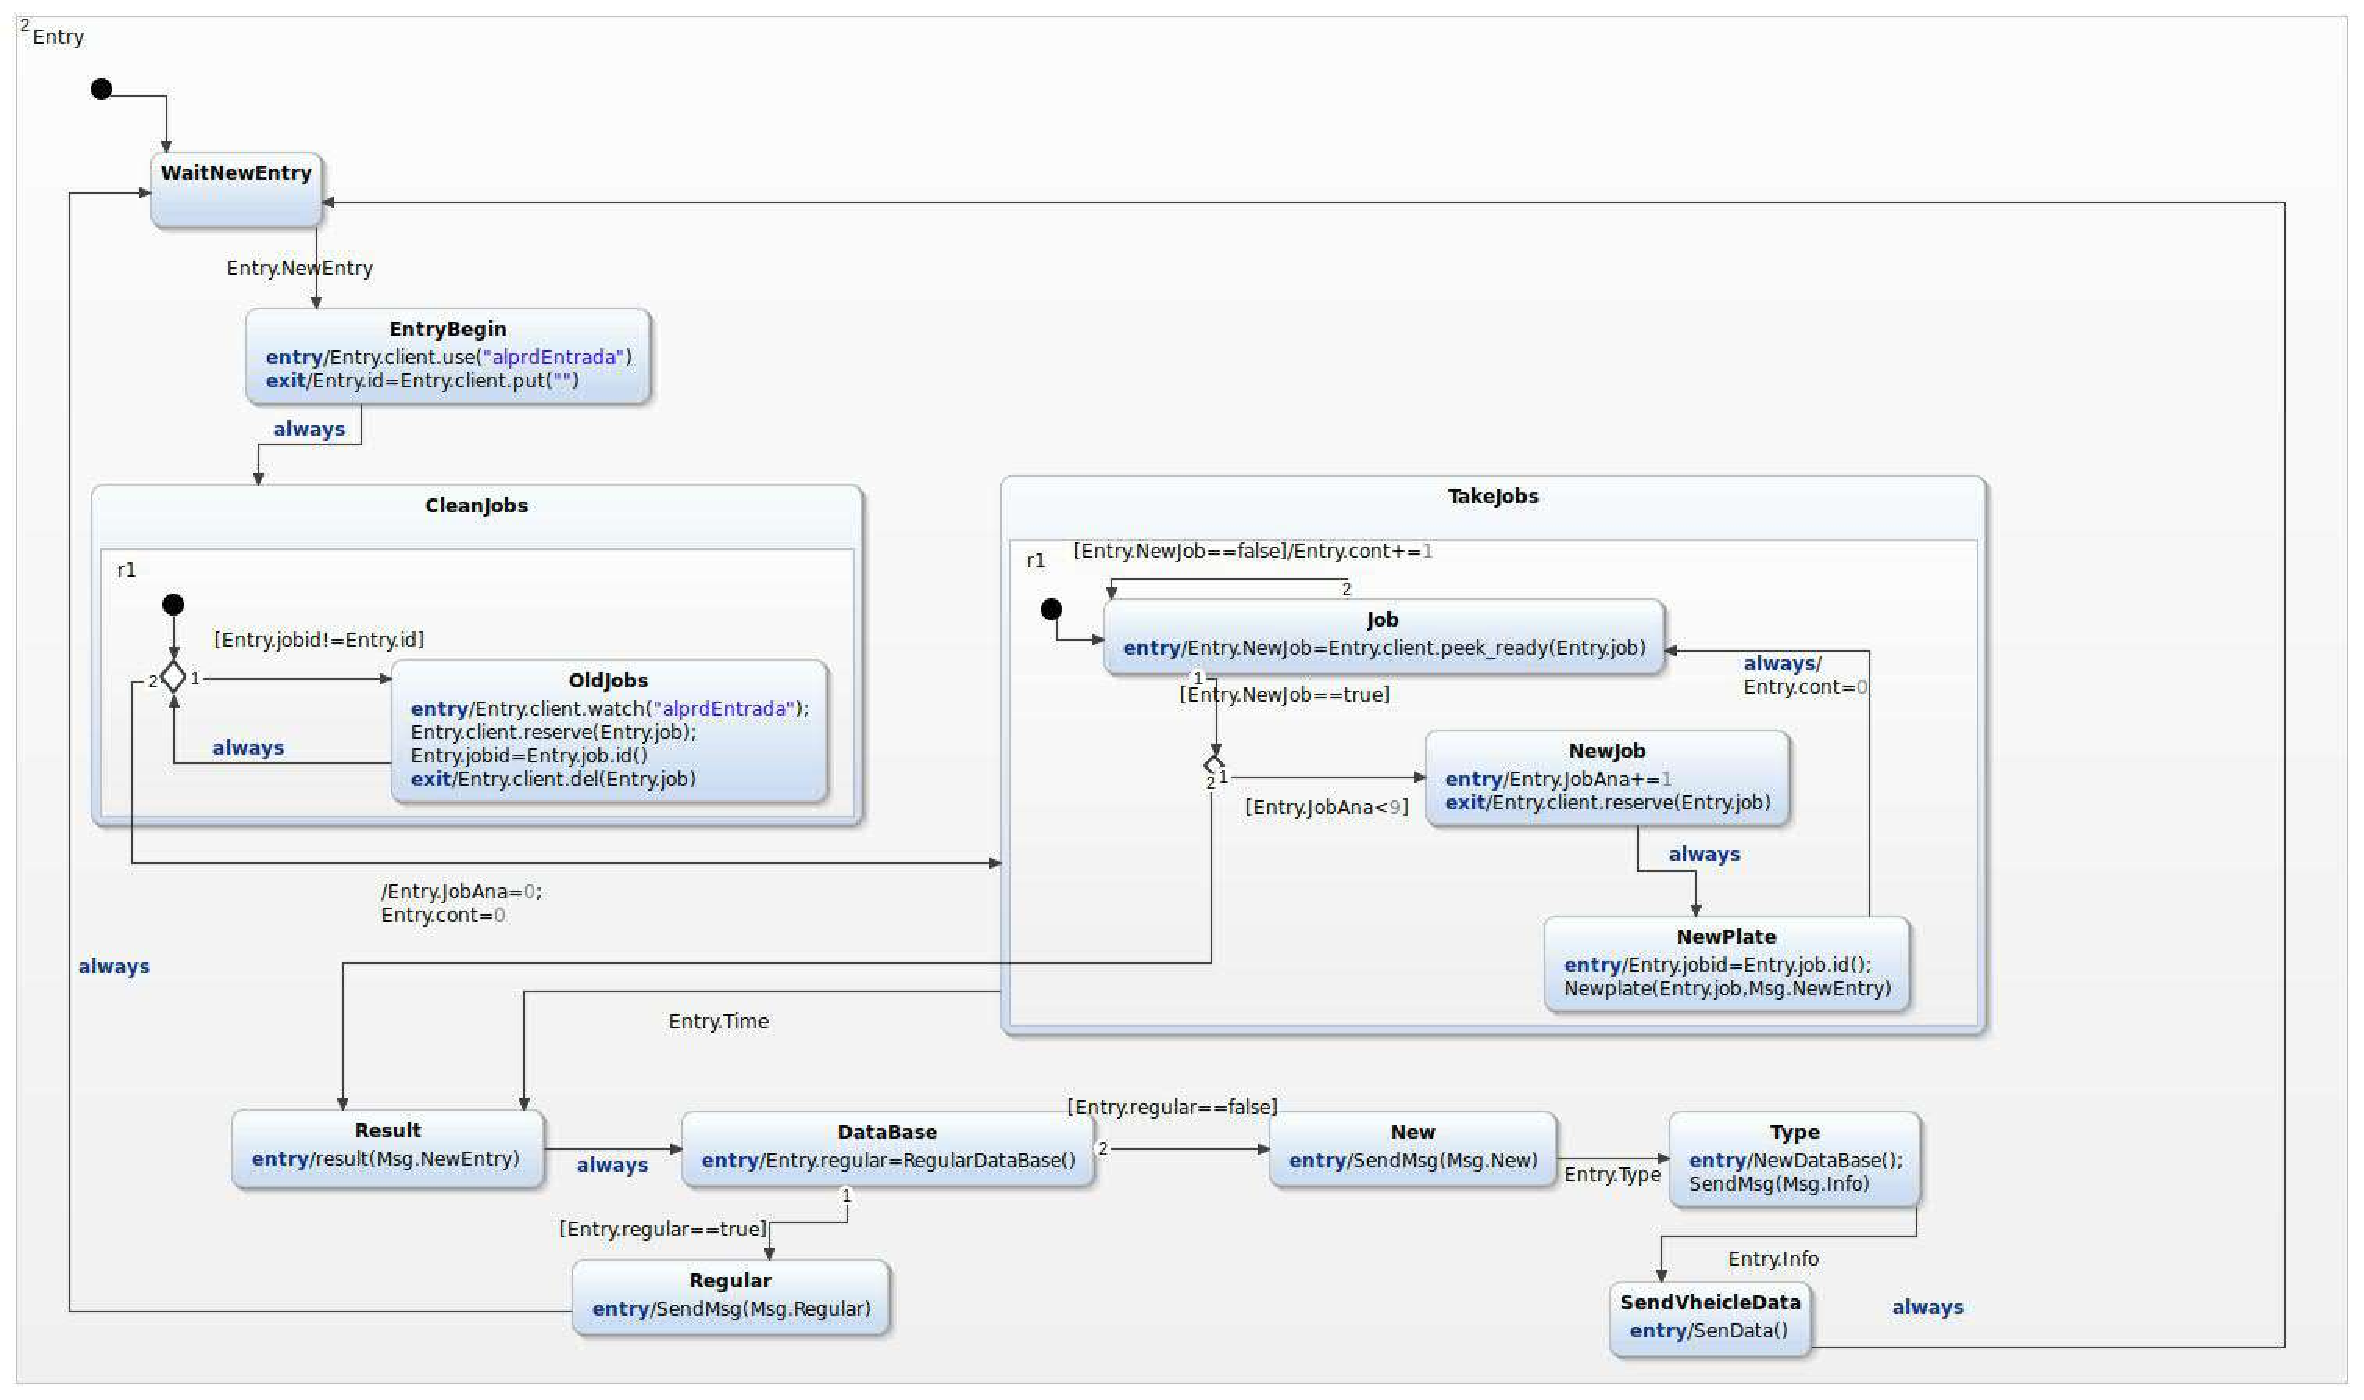
\includegraphics[width=\textwidth]{EntradaUCC.pdf}
	\caption{Procedimiento sobre la Vía de ingreso de la UCC.}
	\label{fig:img_EntradaUCC}
\end{figure}

\begin{figure}[H]
	\centering
	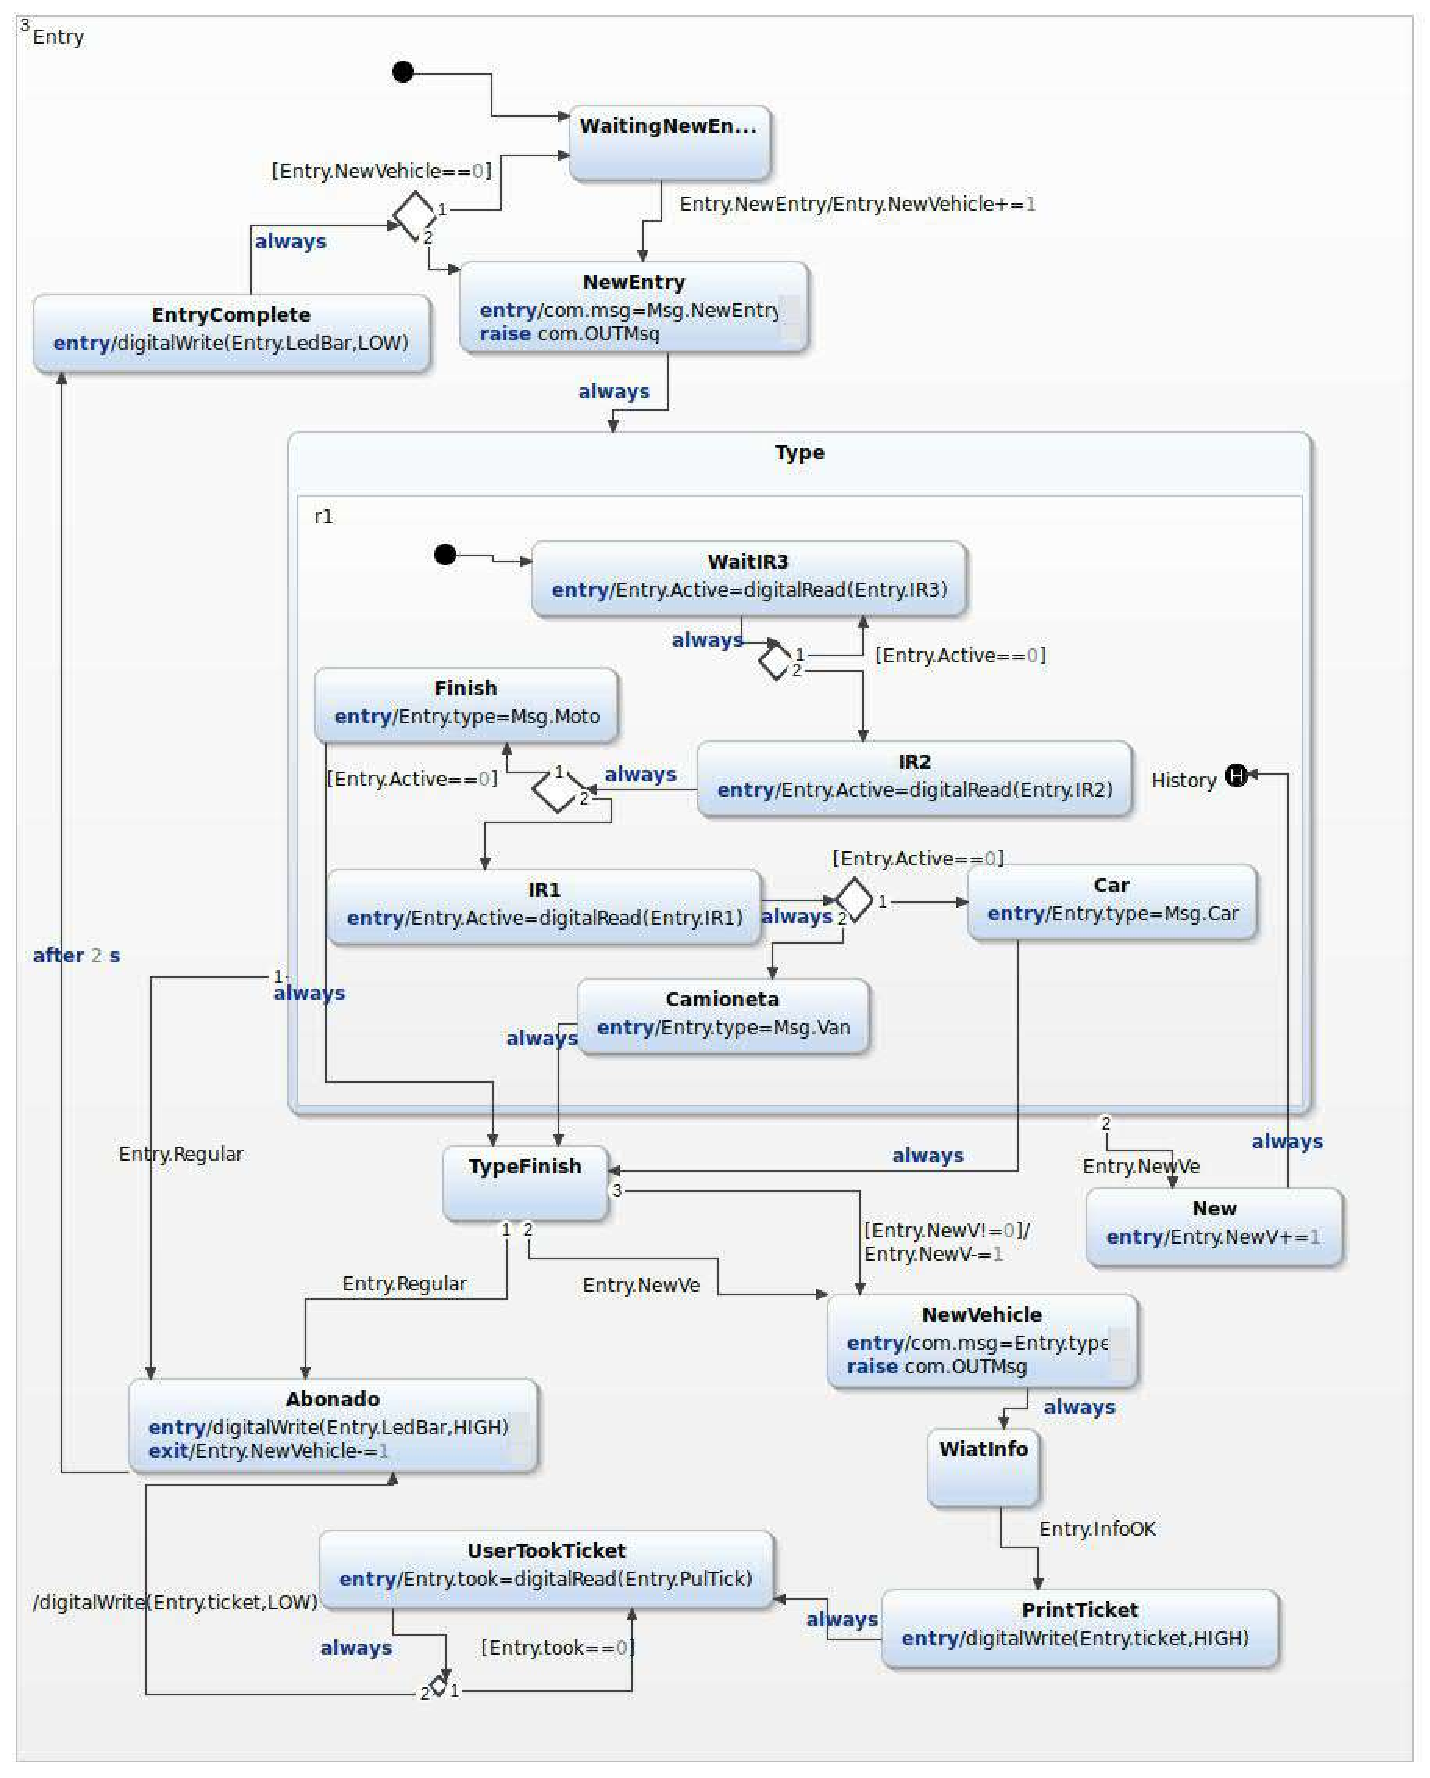
\includegraphics[width=\textwidth]{EntradaPlaca.pdf}
	\caption{Procedimiento sobre la Vía de ingreso de la Placa I/O.}
	\label{fig:img_EntradaPlaca}
\end{figure}


En la vía de ingreso, la placa se encuentra verificando continuamente el estado del detector magnético. Una vez que este se activa, comienza el funcionamiento de la región mostrada en la figura~\ref{fig:img_EntradaPlaca}. La primera acción de la misma es comunicarle a la UCC que un nuevo vehículo ha ingresado al estacionamiento. Al recibir esta información, la UCC levanta el evento ``NewEntry'' y procede con la fase de obtención de la patente.

Para obtener la matrícula, en primera instancia , la UCC inserta un trabajo bandera del cual se guarda el número de ID. Este se utiliza como guía para eliminar todos los trabajos anteriores acumulados en la cola, que poseen un número de ID inferior al mismo, evitando así que se efectúe una lectura errónea. Una vez que estos son eliminados, se procede a analizar los nuevos trabajos que el sistema va agregando a la cola hasta alcanzar una cifra de nueve, o bien, hasta que transcurran dos segundos. Luego, dado que se obtiene un resultado para la patente por cada trabajo analizado, la respuesta a devolver corresponderá a aquel que más veces se presente. Cabe destacar que, de esta manera, el sistema puede obtener diferentes posibles resultados para la misma patente. Por lo tanto, en caso de que se produzca un empate entre la cantidad de ocurrencias de dos (o más) resultados, se elige aquel que presente un valor de confianza mayor. Por otra parte, en caso de que no se logre analizar ningún trabajo, el sistema entrega como respuesta un número de siete cifras que representa un patente provisoria.

Con el resultado de la patente obtenido, la UCC debe verificar si el vehículo que desea ingresar al establecimiento es un cliente nuevo o un abonado. Para realizar esto se implementó una base de datos sencilla basada en MySQL. Este es un sistema de gestión de bases de datos desarrollado en C/C++ bajo licencia dual: Licencia pública general/Licencia comercial, por Oracle Corporation, y está considerada como la base de datos de código abierto más popular del mundo \cite{mysql}.

La base de datos creada consta de tres tablas independientes. En la primera de ellas, denominada ``Regular'', se registran todos los vehículos abonados, es decir, aquellos que pagan una tarifa mensual. En la segunda, llamada ``Parking'', se almacenan todos los automóviles que hayan ingresado al establecimiento y aún no se hayan retirado. Esto implica que, con esta tabla, se puede saber la cantidad de vehículos estacionados dentro del estacionamiento. Por último, la tabla denominada ``History'', lleva un historial de todos los vehículos que han ingresado y salido del establecimiento.

Entonces, para determinar si un vehículo es abonado o no, la UCC verifica si su patente se encuentra en la tabla ``Regular''. La misma se observa en la figura~\ref{fig:img_BDREGULAR}. Luego, se ingresa la información de la patente, la fecha y hora de ingreso a la tabla ``Parking'', la cual se ve en la \hl{figura x10 (poner antes de que se actualice el tipo)}. Por último, se informa a la placa de qué tipo de cliente se trata. En el caso de un abonado, además de la información mencionada, también se añade el tipo de vehículo y el estado del pago a dicha tabla.

\begin{figure}[H]
	\centering
	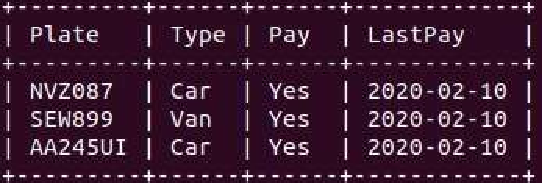
\includegraphics[scale=1]{BDREGULAR.pdf}
	\caption{Tabla ``Regular'' de la base de datos desarrollada.}
	\label{fig:img_BDREGULAR}
\end{figure}

%\begin{figure}[H]
%	\centering
%	\includegraphics[width=\textwidth]{figura x10.pdf}
%	\caption{Tabla “Parking” de Base de Datos(poner q se ve un abonado y un no abonado).}
%	\label{fig:img_}
%\end{figure}

Mientras la placa espera que la UCC envíe la información acerca de la clase de cliente, calcula el tipo de vehículo que intenta ingresar: auto, moto o camioneta. Para ello, se implementa un sistema constituido por tres barreras infrarrojas, las cuales se encuentran dispuestas cada 2.5m. Se determinó que esta debía ser la distancia, a raíz de una investigación realizada sobre el tamaño máximo y mínimo que pueden tener los tres tipos de vehículos a detectar. En cuanto a su funcionamiento, el sistema analiza cuántas de las tres barreras son cortadas simultaneamente por el vehículo que ingresa, cuando la más cercana de ellas a la barrera es activada. En caso de que los tres haces infrarrojos sean interrumpidos, se trata de una camioneta. Por otra parte, si solo los 2 sensores más próximos a la barrera se encuentran activados, es un auto. Finalmente, si no se activa más de una barrera a la vez, el vehículo es una motocicleta. De esta forma, se determina la tarifa que debe abonarse, ya que en muchos estacionamientos del país se cobra un monto diferenciado según el tipo de automóvil.

En el caso de un cliente abonado, luego de enviar la información mencionada anteriormente, la UCC vuelve a quedar a la espera de un nuevo ingreso. Por otra parte, la placa al recibir esta información, descarta el cálculo del tipo y el retiro del ticket, y le permite el ingreso al estacionamiento levantando la barrera. Esto se puede visualizar con el encendido de un led, durante dos segundos, que representa la barrera.

En el caso de un cliente no abonado, luego de informar su clase, la UCC espera recibir el tipo de vehículo para actualizar la tabla de la base de datos. Esto se observa en la \hl{figura x11}. 

%\begin{figure}[H]
%	\centering
%	\includegraphics[width=\textwidth]{figura x11.pdf}
%	\caption{Tabla "parking" con tipo de vehículo actualizado.}
%	\label{fig:img_}
%\end{figure}

Al recibir que se trata de un no abonado, la placa le informa a la UCC el ``tipo'' que determinó, y queda a la espera de la patente y la hora de ingreso. Estos datos se presentarían en el ticket que se le entrega a los usuarios, pero, en este caso, la impresión del mismo se encuentra simulada por el encendido de un led. Por lo tanto, al recibir la información del tipo, la UCC responde con estos datos, terminando su participación en el proceso de entrada. Al recibir dicha información, la placa enciende el led que indica que el ticket fue impreso. 

Por último, para permitir el acceso al establecimiento, el usuario debe retirar el ticket. En este caso, esta acción se encuentra representada por la activación de un pulsador. Entonces, al presionarlo, se lleva a cabo el retiro del ticket, se apaga el led de ticket impreso y se enciende, durante dos segundos, el led que simula la barrera. De esta manera, se concluye el ingreso del vehículo.

Debe tenerse en cuenta que, si se activa el detector magnético mientras está ingresando otro vehículo, esta condición se guarda. Por lo tanto, luego de que se apague el led de barrera, la placa no vuelve a su estado de espera, sino que comienza directamente con el proceso de ingreso pendiente.

Finalmente, en el caso de vehículos que no posean patentes, o que la misma no se haya podido obtener, el sistema igualmente permite el ingreso y se establece una patente provisoria, como se mencionó anteriormente.


\subsection{Vía de egreso}

De manera similar al caso de la vía de ingreso, tanto la Placa I/O como la UCC tienen una región destinada a la salida del vehículo, mientras que el módulo WiFi solo retransmite los mensajes. Ambas regiones pueden visualizarse en las figuras~\ref{fig:img_SalidaPlaca} y~\ref{fig:img_SalidaUCC}, respectivamente.

\begin{figure}[H]
	\centering
	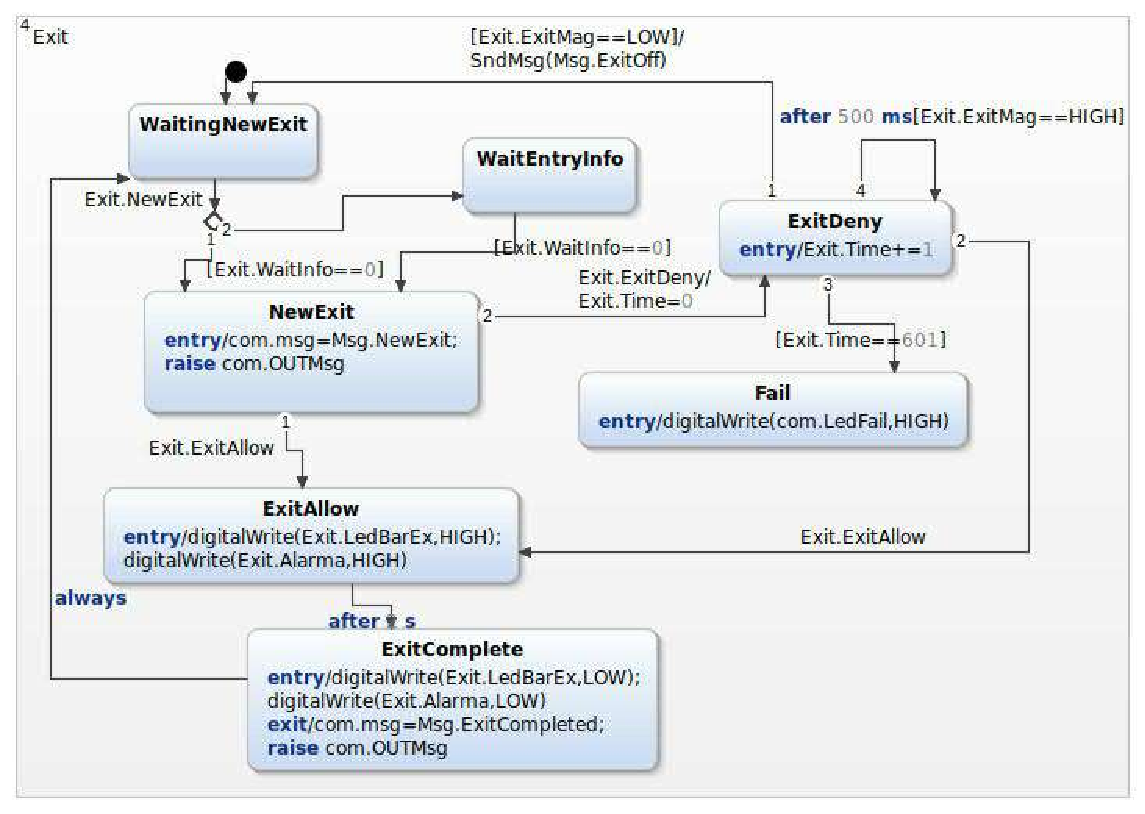
\includegraphics[width=\textwidth]{SalidaPlaca.pdf}
	\caption{Etapa de egreso de la Placa I/O.}
	\label{fig:img_SalidaPlaca}
\end{figure}

\begin{figure}[H]
	\centering
	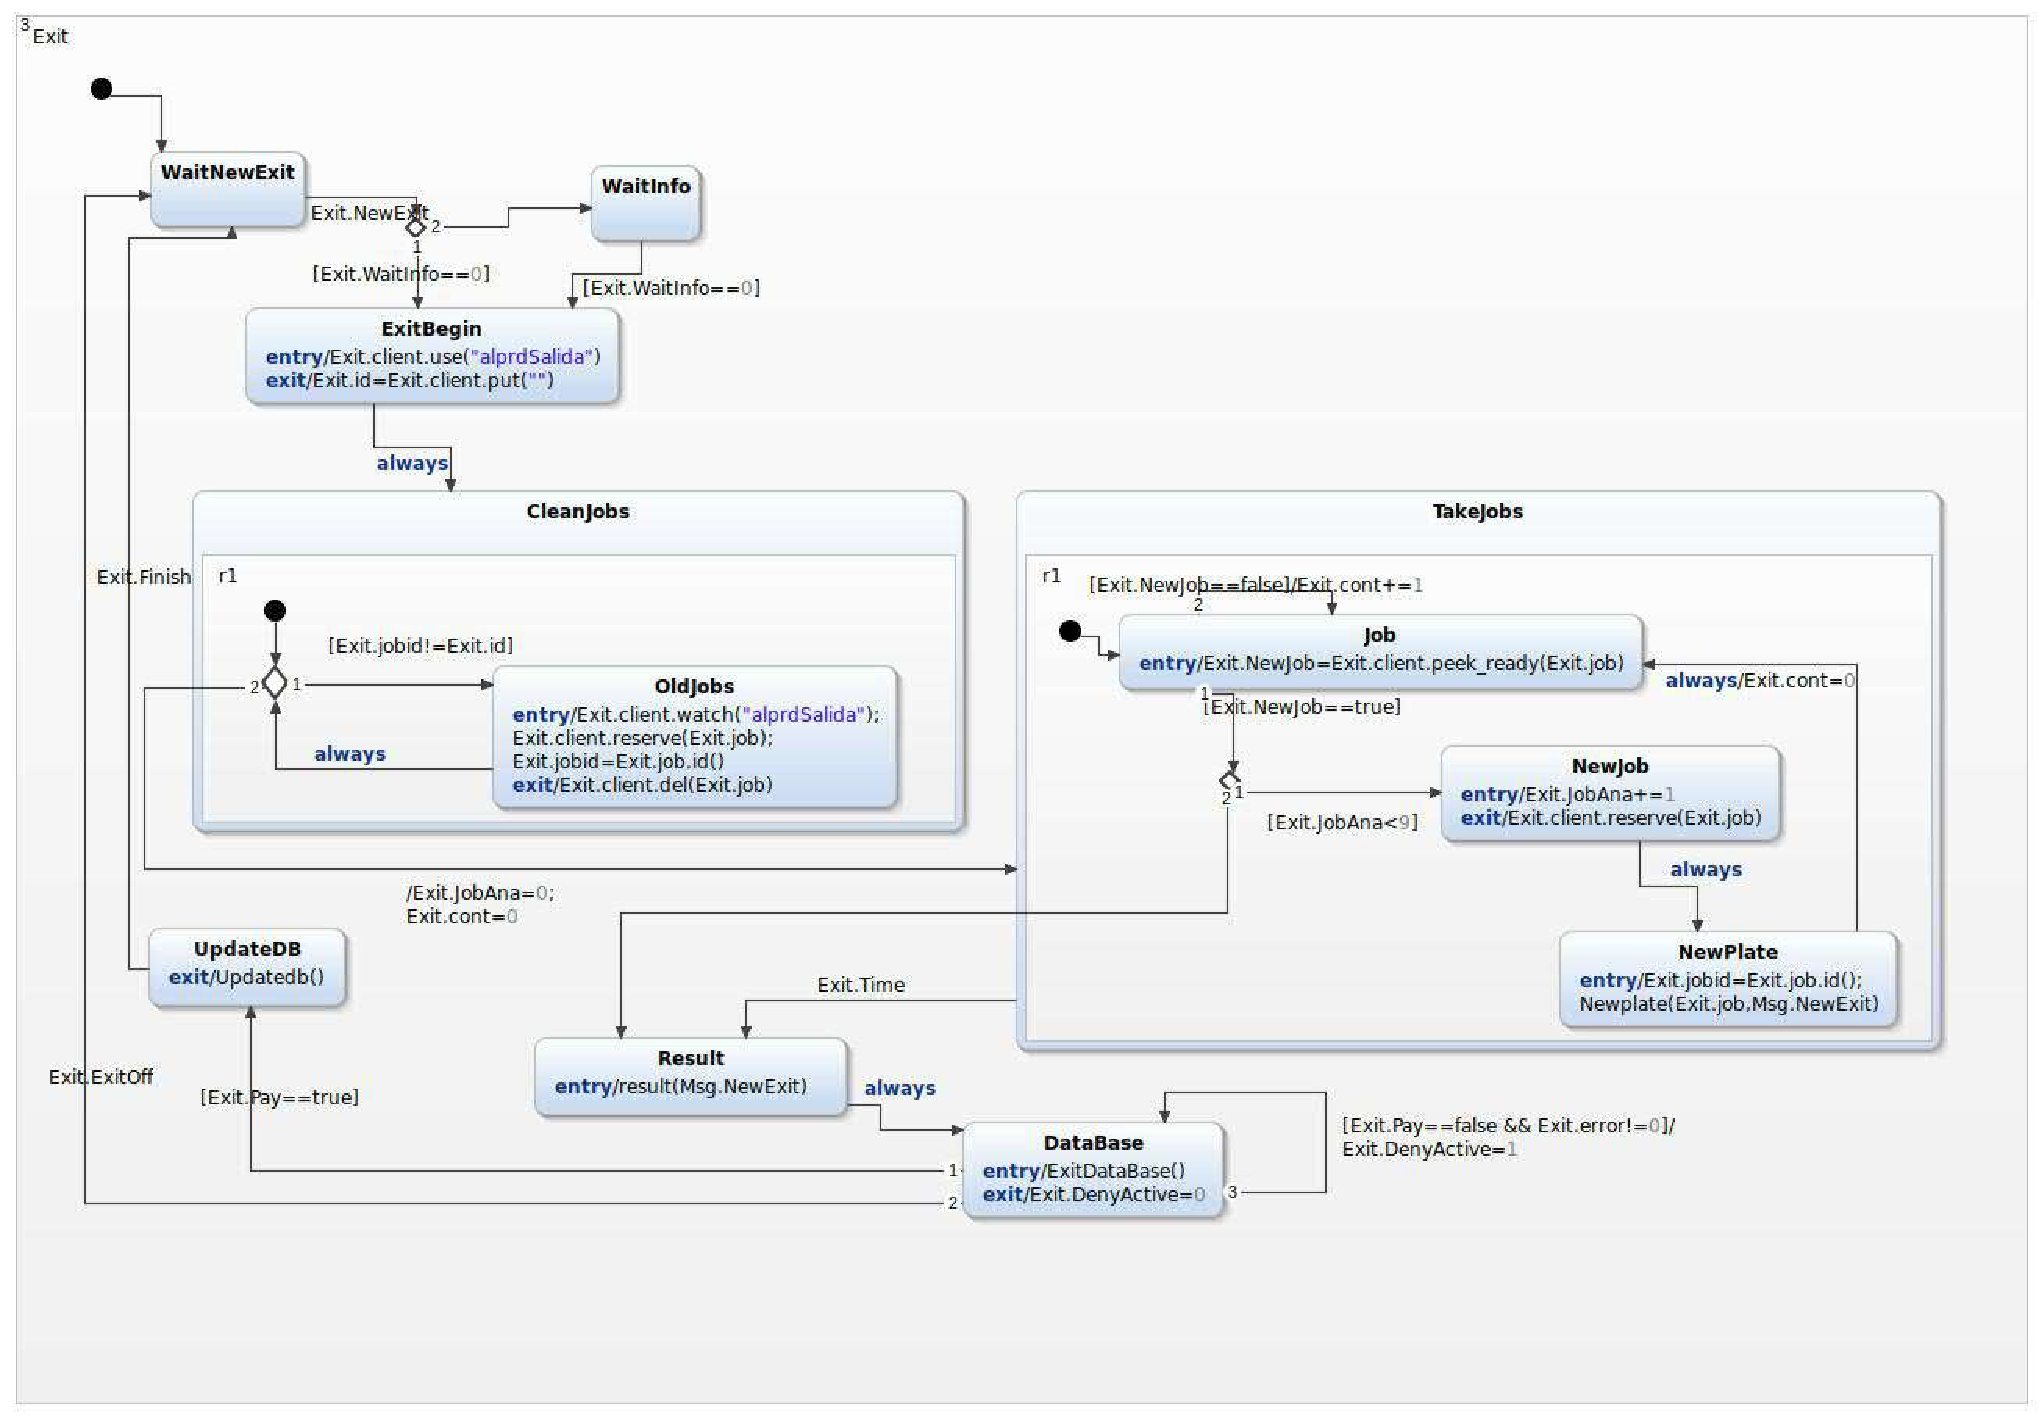
\includegraphics[width=\textwidth]{SalidaUCC.pdf}
	\caption{Etapa de egreso de la UCC.}
	\label{fig:img_SalidaUCC}
\end{figure}

Al igual que en la vía de ingreso, el sistema se encuentra a la espera de la activación del detector magnético. Cuando la Placa I/O verifica que un nuevo vehículo desea retirarse del establecimiento, lo informa a la UCC y se mantiene a la espera de la respuesta de ésta.

La única diferencia con la entrada es que en caso de no detectar ninguna patente, se establece el valor ``NoPlate'' como resultado. 

Al recibir esta información, el proceso seguido por la UCC para obtener la patente del vehículo que activó el sistema es idéntico al de la entrada. La UCC debe verificar que la matrícula detectada se encuentre en la tabla ``Parking'', es decir, que se comprueba que el vehículo haya ingresado. Por lo tanto, en este punto tenemos dos posibilidades:

\begin{enumerate}
	\item \textbf{La patente se encuentra en la base de datos.} En este caso, se verifica si el cliente ya realizó el pago de la tarifa. Con la finalidad de ensayar el prototipo, se diseñó un código que lo simula. En este, se le pide al operario que ingrese la patente, la tarifa y si el pago fue efectuado. De esta manera, se actualiza la información de la tarifa, el estado del pago y la fecha y hora de salida en la tabla “Parking”, de la base de datos. En la \hl{figura x11}, se puede observar que dichos campos se encontraban vacíos, mientras que en la \hl{figura x14} se ve que fueron actualizados. Por lo tanto, la UCC avisa a la placa que el egreso es permitido o denegado dependiendo de esta condición.
	
	\item \textbf{La patente no se encuentra en la base de datos.} En este caso, se informa por pantalla al operario de lo sucedido, y este debe verificar si fue un error en la detección de la patente o no, visualizando el vehículo. En el primer caso, se le pide que ingrese la patente correcta y el sistema la vuelve a buscar en la base de datos, llevando a cualquiera de éstas posibilidades nuevamente. Se destaca que, en el caso de no poder detectar correctamente la patente, si a la entrada se asignó una provisoria, se debe ingresar ese valor. En el segundo caso, se avisa a la placa que el egreso fue denegado.
	\end{enumerate}

%\begin{figure}[H]
%	\centering
%	\includegraphics[width=\textwidth]{figura x14.pdf}
%	\caption{Tabla “Parking” con valores actualizados.}
%	\label{fig:img_}
%\end{figure}

Por lo tanto, luego de verificar en la base de datos, la UCC informa a la placa sobre si la salida es autorizada o no. Esto lleva a dos casos posibles:

\begin{enumerate}
	\item \textbf{Salida autorizada.} En este caso, la placa enciende durante dos segundos el led que simula la barrera de salida, permitiendo el egreso del vehículo. Una vez que se completa el egreso, la placa se lo informa a la UCC, terminando su parte en el proceso y quedando a la espera de un nuevo egreso. De esta manera, al recibir esta información, la UCC elimina al vehículo de la tabla “Parking” y lo agrega a la tabla “History”. Esto se puede observar en las \hl{figuras x15 y x16,} respectivamente. Luego de esta actualización, el proceso actual finaliza y la UCC queda preparada para el arribo de un nuevo vehículo.
	
	%\begin{figure}[H]
	%	\centering
	%	\includegraphics[width=\textwidth]{figura x15.pdf}
	%	\caption{Tabla “Parking” con vehículo borrado.}
	%	\label{fig:img_}
	%\end{figure}
	
	%\begin{figure}[H]
	%	\centering
	%	\includegraphics[width=\textwidth]{figura x16.pdf}
	%	\caption{Tabla “History” con vehículo agregado.}
	%	\label{fig:img_}
	%\end{figure}
	
	
	\item \textbf{Salida Denegada.} Luego de enviar esta información, la UCC se mantiene comprobando de manera continua el estado del pago de la tarifa. Esto se debe a que en el momento en que el cliente realice esta acción, se le autorizará el egreso. En caso de que la salida haya sido denegada por no encontrarse la patente en la base de datos, el sistema se queda a la espera de que el vehículo se retire de la vía de egreso, retrocediendo hacia el interior del establecimiento. Simultaneamente, la placa se encarga de analizar si el vehículo sigue posicionado sobre el detector magnético. En caso afirmativo, el cliente tiene cinco minutos para realizar el pago, si aún no lo hizo, o para retirar el vehículo de la vía de egreso. En la primera situación, al actualizarse el pago, la UCC lo verifica y se procede como en el caso de la salida autorizada. Por otra parte, si el cliente retira el vehículo de la salida, esto se informa a la UCC y el sistema finaliza el proceso, quedando preparado para recibir un nuevo vehículo.
\end{enumerate}

Cabe destacar que, en este caso, no existe la posibilidad de que un segundo vehículo active el detector magnético mientras otro realiza el ingreso. Esto se debe a que el mismo se ubica muy próximo a la barrera, por lo cual va a mantenerse activado por el mismo vehículo hasta el momento en que se retire.



